\section{方法}

本节首先在第~\ref{sec:formulation} 节形式化问题，随后在第~\ref{sec:method_design} 节详细介绍 \our 的设计，最后在第~\ref{sec:learnable} 节说明专用编排器的训练过程。图~\ref{fig:piepine} 给出了方法概览。

\begin{figure*}[t]
    \centering
    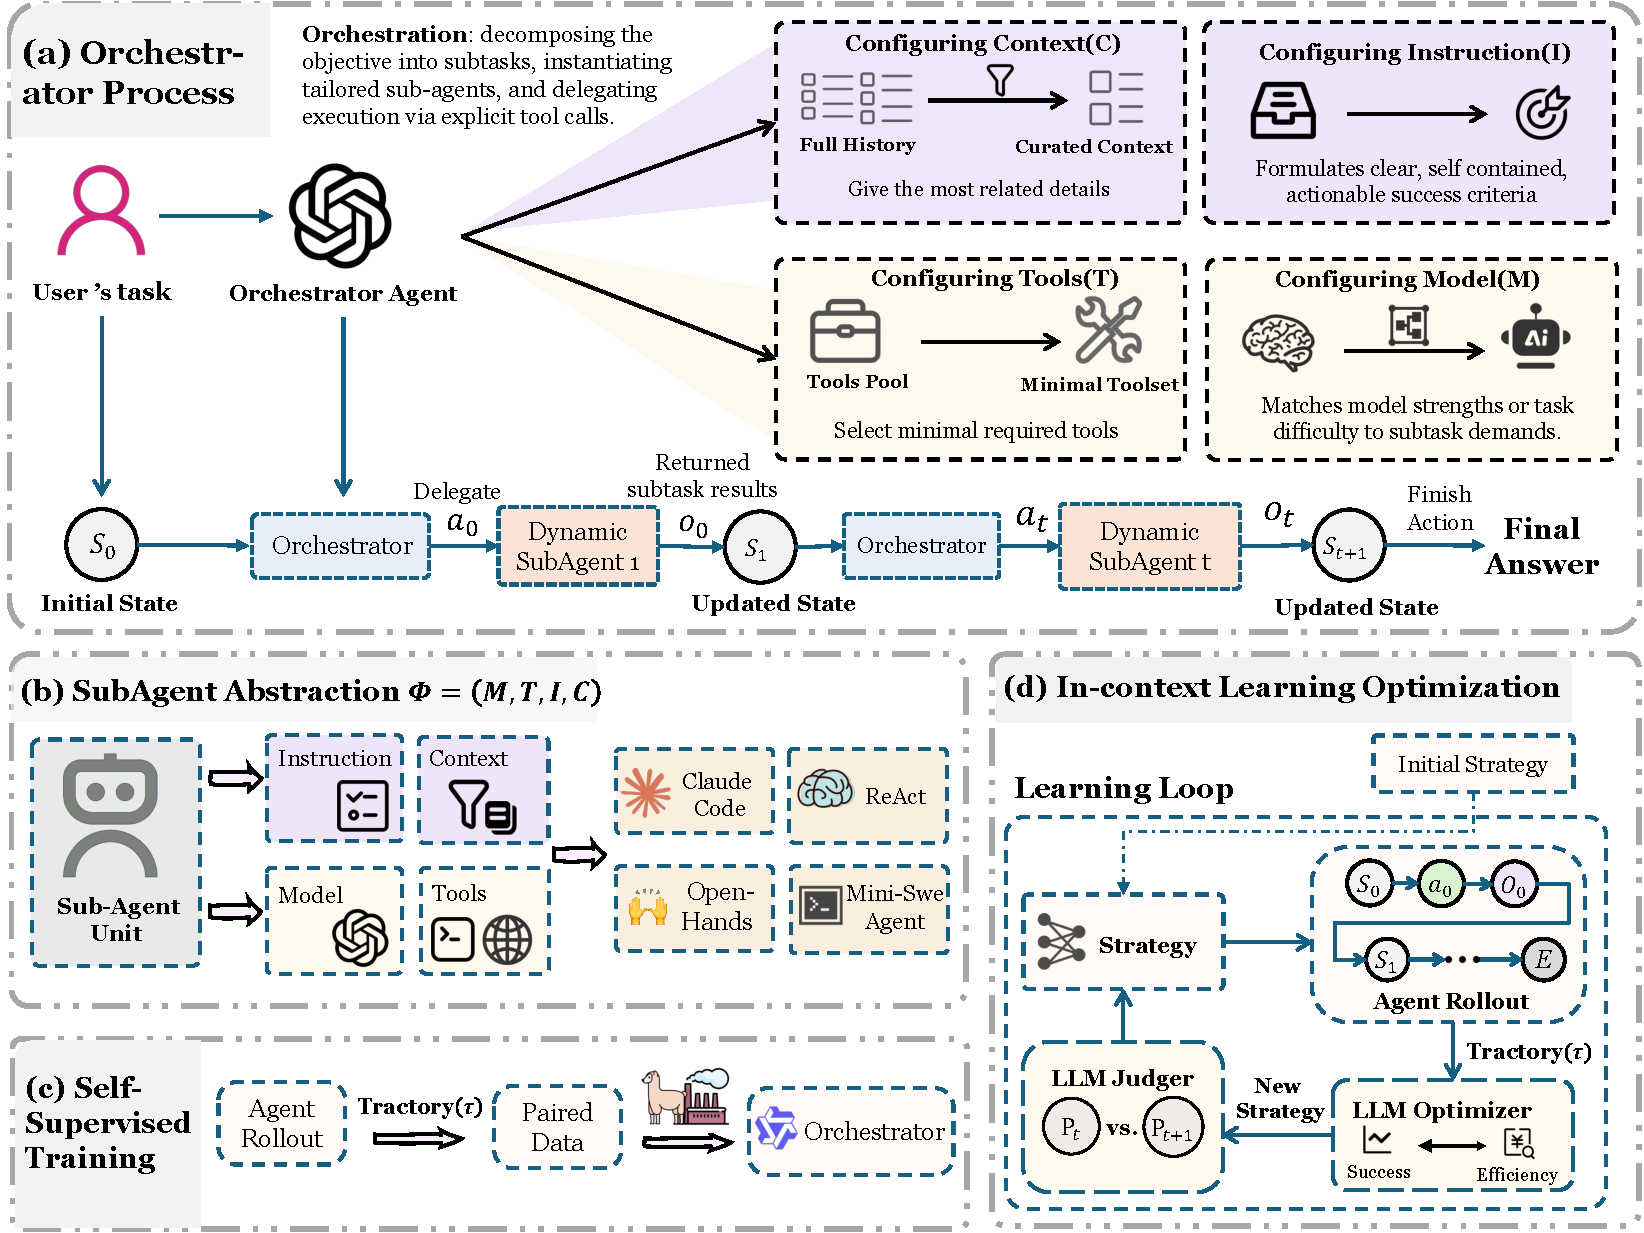
\includegraphics[width=\textwidth]{figures/introduction.pdf}
    \caption{面向复杂长程任务的智能体框架 \our{} 总体设计。编排器通过反复将子任务委派给即时实例化的子智能体来完成用户任务，每个子智能体都由统一四元组 $(I,C,T,M)$ 定义。编排器本身可学习，并能从以往经验中改进任务分解、上下文路由和能力分配。}
    \label{fig:piepine}
\end{figure*}

\subsection{问题形式化}
\label{sec:formulation}
本文主要关注复杂智能体任务。智能体系统通过与环境进行多步交互来完成用户目标 $G$。环境提供\emph{环境级}动作空间 $\mathcal{A}_{\text{env}}$，例如 shell 命令、网页操作和代码编辑，并返回观测、工具输出和错误消息等反馈。因此，一项任务的交互轨迹可定义为：
\[
\tau = (s_0, a_0, o_0, s_1, a_1, o_1, \dots, s_T),
\]
其中，$s_t \in \mathcal{S}$ 表示第 $t$ 步的系统状态，包括累积历史、中间结果与环境反馈；$a_t$ 表示第 $t$ 步采取的动作；$o_t \in \mathcal{O}$ 表示返回的观测。系统按照如下状态转移函数演化：
\[
s_{t+1} = \delta(s_t, a_t, o_t),
\]
其中，$\delta: \mathcal{S} \times \mathcal{A}_{\text{env}} \times \mathcal{O} \rightarrow \mathcal{S}$ 将当前状态、动作和观测映射到下一状态，即把新返回的信息纳入系统内部状态。

\paragraph{子智能体即工具视角。}
我们关注“子智能体即工具”范式。在该范式中，\emph{主智能体}（编排器）既可以直接在环境中行动，也可以通过工具调用把子任务委派给子智能体。相应地，编排器操作一个\emph{系统级}动作空间，通常包含三类动作：(1) 环境动作 $u \in \mathcal{A}_{\text{env}}$；(2) 调用子智能体执行的委派动作（\texttt{Delegate}$(\cdot)$）；(3) 终止动作（\texttt{Finish}）。我们将这一通用编排动作空间记为：
\[
\mathcal{A}_{\text{orch}} \supseteq \mathcal{A}_{\text{env}} \ \cup\ \{\texttt{Delegate}(\cdot),\ \texttt{Finish}(y)\}.
\]
不同系统的主要差异在于如何参数化 \texttt{Delegate}，例如只携带上下文进行委派，或委派给一组固定角色；另一项差异是编排器本身是否也执行环境动作。

我们的目标是最大化任务成功率，并可选择性地权衡执行成本：
\[
\max_{\pi}\ \mathbb{E}\Big[\mathbf{1}\{\text{Success}(G)\}-\lambda\cdot \text{Cost}(\tau)\Big],
\]
其中，$\pi$ 是编排器策略，$\text{Cost}(\tau)$ 可以包括 token 用量、工具调用次数、延迟或货币成本，$\lambda$ 控制成本与性能之间的权衡。

\subsection{\our{}}
\label{sec:method_design}

\paragraph{统一的四元组智能体抽象。}
\our{} 使用统一且与框架无关的抽象对\emph{主智能体和子智能体}建模。我们把一个智能体实例定义为可实例化的四元组：
\[
\Phi = (I, C, T, M),
\]
其中，$I$ 是规定当前目标与成功标准的任务指令；$C$ 是经过筛选、供智能体作出判断的工作上下文；$T$ 是定义智能体动作空间的工具集合；$M$ 是与环境交互的底层模型。该抽象显式分离了两个需要\textit{专门化}的互补维度：\emph{工作记忆} $(I,C)$ 与\emph{能力} $(T,M)$。需要强调的是，我们不把子智能体视为静态实体，而是将其视为可在运行时参数化和创建的\emph{动态}单元。

主智能体（编排器）同样可以表示为四元组 $\Phi^{\text{main}}=(I^{\text{main}},C^{\text{main}},T^{\text{main}},M^{\text{main}})$。区别在于，$T^{\text{main}}$ 提供的是用于编排的\emph{系统工具}，如 \texttt{Delegate} 和 \texttt{Finish}，而不是 $\mathcal{A}_{\text{env}}$ 中的环境工具。

\paragraph{编排器的动作空间。}
基于上述抽象，\our{} 将编排与执行解耦。\our{} 的编排器从不直接执行 $\mathcal{A}_{\text{env}}$ 中的环境动作，而只操作以下两种动作：
\[
\mathcal{A}_{\our} = \{\texttt{Delegate}(\Phi),\ \texttt{Finish}(y)\}.
\]
在第 $t$ 步，编排器采样动作 $a_t \in \mathcal{A}_{\our}$。若 $a_t=\texttt{Delegate}(\Phi_t)$，系统会创建执行器 $A(\Phi_t)$ 来执行子任务并返回观测 $o_t$；若 $a_t=\texttt{Finish}(y)$，交互以最终答案 $y$ 终止。返回的观测通过 $s_{t+1}=\delta(s_t,a_t,o_t)$ 纳入下一状态。

\paragraph{\texttt{Delegate} 与 \texttt{Finish} 的实现。}
我们为 \our{} 的编排器提供两个系统工具：\texttt{Delegate} 和 \texttt{Finish}。\texttt{Delegate} 接收 $\Phi_t=(I_t,C_t,T_t,M_t)$ 作为参数，并据此实例化执行器。该执行器使用模型 $M_t$，只能访问工具集合 $T_t$，且仅以 $(I_t,C_t)$ 为条件执行任务。它向编排器返回结构化观测 $o_t$，通常包括：(1) 简洁的结果摘要；(2) 相关产物，如文件和参考资料；(3) 执行失败时的错误消息或日志。\texttt{Finish} 终止交互并输出最终响应 $y$。

\paragraph{\our{} 的优势。}
我们提出的 \our{} 具有多项关键优势。第一，它会按需为每个子智能体动态配备定制能力，显著提高任务执行准确率。与以往工作~\cite{sun2025scaling, anthropic_claude_code_subagents} 不同，编排器会有意识地向子智能体提供结构良好的上下文。第~\ref{sec:adv1} 节将表明，这种谨慎的上下文管理可以增强模型求解任务的能力。第二，编排器只操作四元组抽象，不依赖子智能体的内部实现。因此，我们可以采用多种子智能体设计，例如简单的 ReAct 方法~\cite{yao2022react} 或 mini-SWE 智能体。第三，编排器可以从大量经验中学习。第~\ref{sec:learnable} 节将进一步说明，这些可学习能力既包括基础任务编排技能，即做什么、依据哪些信息以及使用哪些工具，也包括自适应模型路由等高级能力，其目标可以是通过选择最合适的模型来平衡性能与成本。

\subsection{可学习的编排器}
\label{sec:learnable}

在 $\mathcal{A}_{\our}=\{\texttt{Delegate}(\Phi),\texttt{Finish}(y)\}$ 下，编排任务可以表述为学习结构化动作上的策略：
\[
\pi_\theta(a_t \mid s_t),\quad a_t\in\mathcal{A}_{\our}.
\]

由于委派参数 $\Phi_t=(I_t,C_t,T_t,M_t)$ 是显式可用的，学习可聚焦于两个互补维度：(1) \textbf{任务编排}，决定做什么、使用哪些上下文以及采用哪些工具；(2) \textbf{模型路由}，选择 $M_t$，即要调用的模型，以平衡性能与成本。下面分别介绍这两种学习范式。

\paragraph{用于任务编排的监督微调（SFT）。}
给定专家编排轨迹 $\{(s_t,a_t^\star)\}$，我们通过行为克隆微调编排器：
\[
\theta^\star = \arg\max_{\theta}\ \sum_{t} \log p_{\theta}(a_t^\star \mid s_t),
\]
其中，$a_t^\star$ 是专家动作，可以是 $\texttt{Delegate}(\Phi_t^\star)$ 或 $\texttt{Finish}(y^\star)$。在我们的设置中，SFT 主要蒸馏\emph{任务编排}能力：改善子任务分解与 $(I_t,C_t,T_t)$ 的合成，从而为每一步生成更好的工作记忆和更合适的工具子集。本文优先展示训练专用编排器的潜力，因此采用直接的 SFT 方法。其他工作也可以使用 GRPO~\cite{shao2024deepseekmath} 等训练方法来增强任务编排能力。

\paragraph{用于成本感知编排的迭代式上下文内学习。}
除更新参数外，我们还可以通过迭代交互学习编排器的\emph{指令}（提示词），在不改变模型权重的情况下优化编排。具体而言，我们把编排器指令 $I^{\text{main}}$ 作为可学习对象，在环境中运行 \our{}，收集轨迹 $\tau=\{(s_t,a_t,o_t)\}_{t=0}^{T}$ 以及任务性能和执行成本等结果指标。随后，优化模型分析这些轨迹，并提出提示词修改 $\Delta I$ 来更新指令：
\[
I^{\text{main}}_{k+1} = \textsc{Optimize}\bigl(I^{\text{main}}_{k},\ \tau_k,\ \text{Perf}(\tau_k),\ \text{Cost}(\tau_k)\bigr),
\]
其中，$k$ 表示优化轮次。系统在环境中使用更新后的编排器反复执行 $N$ 轮，以改进成本感知的编排行为，例如模型选择、路由决策和工具使用模式，并寻找性能与成本之间的帕累托有效权衡。
